\chapter{Newton's law and Dynamical system}Newtons laws of motion describes how  matter behaves in the universe. These are the  three physical laws that, together, laid the foundation for classical mechanics. They describe the relationship between a body and the forces acting upon it, and it's motion in response to those forces. In describing motion it is essential to  specify a reference system . These are the physico-mathematical structures that have the purpose of allowing the objective description, also from a quantitative viewpoint, of physical phenomena that are observed in nature.
\subsubsection{Inertial frames of reference}
Inertial frames are related by a constant velocity along any axis. An object is at rest in an inertial frame when it’s position in space does not change with time.
\subsubsection{Non-Inertial frames of reference}
These are the accelerated frame of reference.
\\\\ It is always possible to find a co-ordinate system with respect to which isolated bodies move uniformly. This is the essence of Newton's first law of motion.


\section{First Law}
Newton's first law of motion is the assertion that inertial systems exist. Newton's first law is part definition and part experimental fact. Isolated bodies move uniformly in inertial systems by virtue of the definition of an inertial system. In contrast, that inertial systems exist is a statement about the physical world.
\begin{definition}
	Every body continues in it's state of rest, or of uniform motion in a straight line, unless it is compelled to change that state by forces impressed upon it.
	\begin{align*}
	\text{If ,} \ F_{ext}&=0 \Rightarrow V= Constant.
	\end{align*}
\end{definition}
After a bus or train starts, the acceleration is often so small we can barely perceive it. We are often startled because it seems as if the station is moving in the opposite direction while we seem to be at rest. Newton's First Law states that there is no physical way to distinguish between whether we are moving or the station is moving, because there is nearly zero total force acting on the body. Once we reach a constant velocity, our minds dismiss the idea that the ground is moving backwards because we think it is impossible, but there is no actual way for us to distinguish whether the train is moving or the ground is moving.
\section{Second Law}
Unlike first law of motion , the Newton's second law of motion is more quantitative and it is used in calculations involving the motion of particles.
\begin{definition}
	The second law states that the net force on an object is equal to the rate of change  of it's linear momentum $\vec{p}$ in an inertial reference frame,
	\begin{align*}
	\vec{F}&=\frac{d \vec{P}}{d t}=\frac{d(m \vec{v})}{d t}\\
	&=m \frac{d(\vec{v})}{d t}+\vec{v} \frac{d(m)}{d t}\\
	&=m \frac{d(\vec{v})}{d t} \qquad (\text{Iff mass is a constant})
	\end{align*}
	
	The second law can also be stated in terms of an object's acceleration. 
\end{definition}
A force ${F}$ on a body of mass $m$ is ${F}= {F}_{i}$, where ${F}_{i}$ is the $i$ th applied force. If a is the net acceleration, and ${a}_{i}$ the acceleration due to ${F}_{i}$ alone, then we have,\\(In most of the cases, mass is a constant quantity then we take the assumption  that mass is a constant.)
\begin{align}
{F}&=\Sigma {F}_{i}=\Sigma m \vec{a}_{i} \notag\\
&=m {\Sigma}\vec{a}_{i}=m \vec{a} \quad (\text{Can be used only if mass is constant.})\\
\vec{a}&=\frac{d \vec{v}}{d t}=\frac{d^{2} \vec{x}}{d t^{2}}\qquad (\text{Acceleration.}  )\notag\\
{F}&=m \frac{d^{2} \vec{x}}{d t^{2}}\label{newtons1}
\end{align}
\begin{center}
	\framebox{
		\parbox[t][1.5cm]{4cm}{
			
			\addvspace{0.2cm} \centering 
			
			${F}=m {a}$\\ \vspace{0.2cm}
			${F}=m \frac{d^{2} \vec{x}}{d t^{2}}$ } }
\end{center}
In cartesian coordinate system, the components of force, $F$, can be written as,
\begin{center}
	\framebox{
		\parbox[t][1.5cm]{6cm}{
			
			\addvspace{0.1cm} \centering 
			
			\begin{align*}
			F_{x}&=m \frac{d^{2} x}{d t^{2}} \quad;\quad
			F_{y}=m \frac{d^{2} y}{d t^{2}} \quad;\quad
			F_{z}=m \frac{d^{2} z}{d t^{2}}\qquad
			\end{align*} } }
\end{center}\vspace{0.2cm}
The right-hand-side of Newton's Second Law is the product of mass with acceleration. Acceleration is a mathematical description of how the velocity of a body changes. Knowledge of all the forces acting on the body enables us to predict the acceleration. Equation.\ref{newtons1} is known as the equation of motion. Once we know this equation we may be able to determine the velocity and position of that body at all future times. 
\section{Third Law}
The fact that force is necessarily the result of an interaction between two systems is made explicit by Newton's third law. 
\begin{definition}
	Third law states that forces always appear in pairs . If body $b$ exerts force ${F}_{a}$ on body $a$, then there must be a force ${F}_{b}$ acting on body $b$, due to body $a$, such that $${F}_{b}=-{F}_{a} .$$ There is no such thing as a lone force without a partner.
\end{definition}
Newton's third law provides such a test. If the acceleration of a body is the result of an outside force, then somewhere in the universe there must be an equal and opposite force acting on another body.   If $\vec{F}_{12}$ be force on an object 1 due to an object 2, and $F_{21}$ be force on 2 due to 1 then,
$$
\vec{F}_{12}=-\vec{F}_{21}
$$
\section{Application of Newton’s Law of Motion}
\subsection{Free body diagram}
\begin{enumerate}
	\item Mentally divide the system into smaller systems, each of which can be treated as a point mass.
	\item Draw force diagram for each mass by considering the body by a point  and draw foce vector on the mass for each mas acting on it.
	\item Assign coordinates to the system of interest. The coordinate system must be an inertial frame.
	\item Assign positive values to all rotations, displacements, velocities, linear velocities, and rotational velocities, and all type of external forces in the problem.
	\item write it's  constraint equation. ( In many problems the objects are constrained to move.)
	\item Using all the force equations and constraint equations find every unknowns of the system.
\end{enumerate}
\section{Dynamical systems}
We start with a very broad definition of a dynamical system and introduce the key theoretical concepts of phase space and fixed points (or limit cycles). While the definition may not cover all dynamical systems, it does cover a whole variety systems of interest to us. We give examples of systems with very simple dynamics to begin with and prepare ground for the treatment of more complicated systems which may not be analytically solvable.
\section{ Dynamical systems of order n}
$\text { A dynamical system of order } n \text { is defined as follows: }$
\begin{enumerate}
	\item The state of the system at any time $t$ is represented by $n$-real variables
	$$
	\left\{x_{1}, x_{2}, x_{3}, \ldots, x_{n}\right\} \Rightarrow \vec{r}
	$$
	as coordinates of a vector $\vec{r}$ in an abstract $n-$ dimensional space. We refer to this space as the state space of simply phase space ${ }^{1}$ in keeping with its usage in Hamiltonian dynamics. Thus the state of the system at any given time is a point in this phase space.
	\item The time evolution of the system, motion is represented by a set of first order equations- the so called "equations of motion":
	\begin{align}
	\frac{d x_{1}}{d t} &=v_{1}\left(x_{1}, x_{2}, \ldots, x_{n}, t\right) \\
	\frac{d x_{2}}{d t} &=v_{2}\left(x_{1}, x_{2}, \ldots, x_{n}, t\right) \\
	\frac{d x_{n}}{d t} &=v_{n}\left(x_{1}, x_{2}, \ldots, x_{n}, t\right)
	\end{align}
	or simply
	$$
	\frac{d \vec{r}}{d t}=\vec{v}(\vec{r}, t)
	$$
	where
	$$
	\vec{v} \Rightarrow\left\{v_{1}, v_{2}, \ldots, v_{n}\right\}
	$$
	is called the velocity function. While we use the notation $x$ and $v$ in analogy with mechanics, they do not always have the usual meaning of position and velocity.
\end{enumerate}
The statements 1 and 2 together define  $\textbf{a dynamical system of order n}$.\\
 If the velocity function does not depend on time explicitly, then the system is timeindependent or autonomous. The set of all possible motions in called \textbf{phase flow}.\\
We also require that the solution to be unique which requires $\vec{v}$ to obey certain conditions. Without going to mathematical details, it suffices to say that the solution of the differential equations in (1.5) are unique if the velocity vector $\vec{v}$ is a continuous function of its arguments and at least once differentiable. With the time evolution, the initial state of the system (denoted by a point in the phase space) evolves and follows a continuous trajectory which we shall call a \textbf{phase curve} which may be closed or open. Distinct phase curves are obtained when the initial state of the system is specified by a point which is not one of the points on the other trajectory. This leads to an important fact that two distinct trajectories can not intersect in a finite time period. The no intersection of phase space trajectories has to do with the fact that the evolution is deterministic. This is an important concept to which we shall return later.
\section{ First order systems}
This is the simplest case of a dynamical system. The equation of motion $^{2}$ is given by
$$
\frac{d x}{d t}=v(x, t)
$$
where $v$ is the velocity function. For any given $v(x, t), x(t)$ is completely determined given $x(t)$ at some $t=t_{0} .$ If, in particular, the system is autonomous, or $v$ is not explicitly dependent on time then the solution can be written as,
$$
t-t_{0}=\int_{x\left(t_{0}\right)}^{x(t)} \frac{d x^{\prime}}{v\left(x^{\prime}\right)}
$$
Thus the solution $x(t)$ depends only on the difference $\left(t-t_{0}\right)$. Thus the time evolution of the system depends entirely on the time elapsed no matter where the origin of time is fixed.
\begin{example} \textbf{ Radio-activity }
 A classic example of a dynamical system of first order is the Radio-active decay of a nucleus modelled by the equation
 $$
 \frac{d N}{d t}=-\sigma N
 $$
 where $N$ is number of nuclei present at some time $t$. The solution of course is well known,
 $$
 N(t)=N_{0} \exp \left\{-\sigma\left(t-t_{0}\right)\right\}
 $$
 where $N_{0}$ is the number of unstable nuclei present at $t_{0}$.
\end{example}
\begin{example}\textbf{ Spread of epidemics}
	Unlike radio-decay, here the growth is usually exponential at least in the initial period. If $\sigma$ is an explicit function of time, as in the case of diseases one may obtain a power-law growth instead of exponential growth. A case which has been studied in detail is the threat of AIDS which has devastated many parts of Africa and is threatening many other countries like India.
	
	In an effort to make quantitative assessment of the threat, efforts have been made to look at the reliable data compiled by Centres for Disease Control in the USA as a function of time. If $I$ is the number of infected persons in a population of size $N$, then the rate of change of $I$ may be given by
	$$\frac{d I}{d t} \approx \alpha I$$
	which gives rise to exponential growth in the initial phases which is usually true in an epidemic. However, it has been observed that in the case of AIDS that the growth shows a cubic dependence on time and not exponential. How is this achieved? Suppose the relative growth rate $\alpha$ is not a constant in time but a decreasing function of time, say,
	$$
	\alpha=m / t
	$$
	where $m$ is a constant. Then the equation may be written as
	$$
	\frac{d I}{d t} \approx m I / t
	$$
	which has a power law solution, namely,
	$$
	I=I_{1} t^{m}+I_{0}
	$$
	It turns out that for AIDS $m=3$.
\end{example}
\begin{example}\textbf{ Population growth}
	A similar exponential growth also occurs in the population growth of various species. When 24 wild rabbits from Europe, not indigenous to Australia, were introduced in Australia they had a disaster on hand. With abundant food with no natural enemies they were in millions within a few years. The impact was so deep
	and widespread that it was called a national tragedy. Since the birth rate is proportional to the size of the population, one gets an equation of motion
	$$
	\frac{d N}{d t}=\sigma N
	$$
	which is similar to radioactive decay equation, but with a positive sign indicating an exponential growth ( $\sigma$ is positive).
	
	The population problem, however, gets more complicated when considerations such as food and predators are introduced.
\end{example}
\begin{example}\textbf{ a non-linear equation}
	The equations of motion can, except in simple situations, get extremely complicated and the solutions are often not easy to obtain. However many qualitative features of a dynamical system may be obtained without actually solving the equations of motion. We will illustrate this with an example below- Consider the equation
	$$
	\frac{d x}{d t}=v(x)=-x\left(1-x^{2}\right)
	$$
	which is similar to the radioactive decay problem with a nonlinear term added. 
\end{example}
Let us look at the properties of the velocity function:\\
\begin{itemize}
	\item The system is autonomous- no explicit time dependence.
	\item The velocity function has zeros at $x_{k}=0, \pm 1-x_{k}$ are the roots of $v(x)$. If the system is at $x_{k}$ at any time, it will continue to remain there for all times. $x_{k}$ are therefore called \textbf{fixed points}. The system is said to be in \textbf{equilibrium} when it is at a fixed point.
	\item The phase space is one dimensional. The phase flows may be indicated by a set of arrows, for example, pointing left(right) if the sign of $v(x)$ is positive(negative) and whose length is proportional to the magnitude of $v(x)$ as shown in figure below. For reference we have also shown $v(x)$ as a function of $x$. The $\mathrm{x}$-axis is the one dimensional phase space of the system.\\
	\begin{figure}[H]
		\centering
		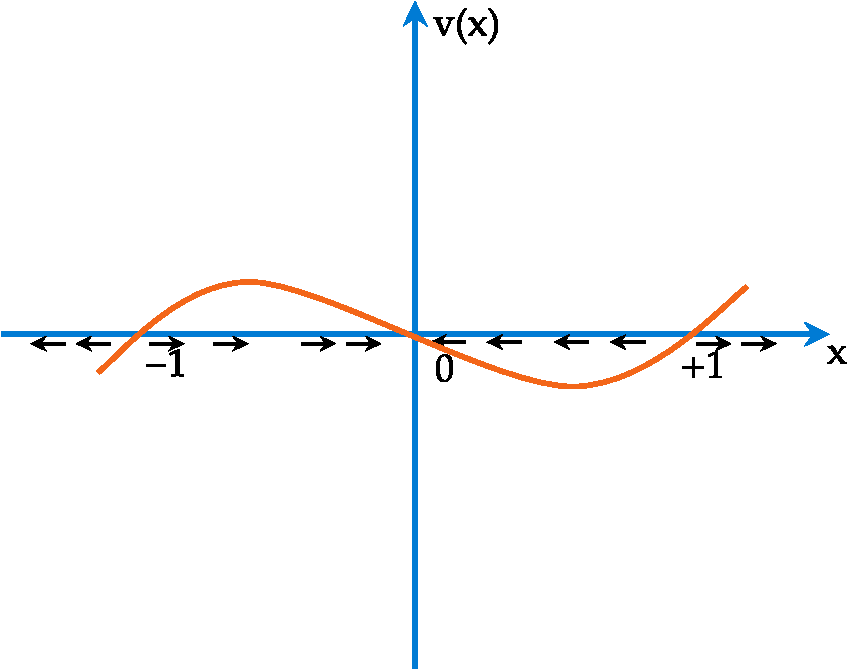
\includegraphics[height=5cm,width=5cm]{diagram-20220214-crop}
		\caption{}
		\label{}
	\end{figure}
\end{itemize}
\textbf{ Properties of Fixed Points}
\begin{itemize}
	\item  The set of zeros of the function $v(x)$ are called the fixed points of the system. The fixed points divide the phase space into several regions.
	\item $x_{k}$ is \textbf{a stable fixed point or sink} if the flow is directed towards the fixed point, otherwise $x_{k}$ is an \textbf{unstable fixed point or repellor.} In the above example obviously $x_{k}=0$ is a stable fixed point where as $x_{k}=\pm 1$ are unstable. It is easy to see that the system evolves towards stable fixed point and away from an unstable fixed point. That is, if $x_{0}$ is a fixed point then define
	$$
	\lambda=\left.\frac{d v}{d x}\right|_{x_{0}}
	$$
	If $\lambda<0$ the fixed point is stable otherwise it is unstable. $\lambda$ is called the characteristic value or some times called Lyapunov exponent.
	\item A fixed point may be both stable and unstable, ie., the neighbouring states approach the fixed point on one side but leave from the other side. We call this a \textbf{saddle point}. This property leads to the so called structural instability, that is even a small perturbation some time can change the nature of fixed point. For example analyse the system with $v(x)=x^{2}$.
	\item The system can not cross a fixed point, by definition. The motion is therefore bounded by the fixed point or fixed points. A system which starts out in the open interval between fixed points remains there for arbitrarily long periods of time. These intervals are therefore called invariant sets. In the example- 4 above the invariant sets are $(-\infty,-1) ;(-1,0) ;(0,1) ;(1, \infty)$
\end{itemize}
Often the motion may be terminating. The terminating motion happens when at some time $t$ the solution of the differential equation is undefined.
\section{ Second order systems}
If the nonlinear differential equation under investigation is of second order and does not contain the independent variable time $t$ explicitly, then it is possible to extract some information regarding the properties of the solution by a geometrical method without actually going into tedious solution of the equation. The dynamical systems whose equations of motion do not involve time $t$ explicitly are called 'autonomous systems'. The equations of motion of second order autonomous systems have the general form
$$
\ddot{x}+g(\dot{x})+f(x)=0
$$
If the velocity $(\dot{x})$ of system is treated as other independent variable and denoted by $y(=\dot{x})$. then equation (1) may be reduced to two first order differential equations as\\
$$\begin{aligned}
	&\frac{d x}{d t}=y \\
	&\frac{d y}{d t}=-[g(y)+f(x)]
\end{aligned}$$
 Equations represent special case of more general system \\
 $$\begin{aligned}
 	&\frac{d x}{d t}=P(x, y) \\
 	&\frac{d y}{d t}=Q(x, y)
 \end{aligned}$$
 $\text { where } P(x, y) \text { and } Q(x, y) \text { are the functions of variables } x \text { and } y \text {. }$\\
Thus Phase space is the superposition of position and momentum space and in phase space the position and velocity coordinated are treated on equal footings.\\
$$\frac{dy}{dx}=-\frac{g(y)+f(x)}{y},y\neq0$$
This differential equation defines a definite curve in the phase space.This curve is called phase tajectory or simply trajectory of the system in the phase space.The phase trajectory is defined by general equations\\
$$\frac{dy}{dx}=\frac{Q(x,y)}{P(x,y)}$$
\subsection{Illustration of phase trajectories}
\textbf{1-Linear harmonic oscillator}\\
The differential equation of linear harmonic oscillator is\\
$$m\frac{d^2x}{dt^2}+kx=0,\frac{dx}{dt}=y$$
These equations may be expressed as \\
$$\frac{dy}{dt}+\frac{k}{m}=0, \frac{dx}{dt}=y$$
Then $$\frac{dy}{dx}=-\frac{kx}{my}$$
or $$mydy+kxdx=0$$
Integrating\\
$$\frac{my^2}{2}+\frac{kx^2}{2}=C$$
The arbitrary constant C is determining by requiring that $x=x_0$ at y=0;This fixes the total energy of the oscillator and C is given by\\
$$ C=0+\frac{kx_0^2}{2}=E$$
Now the equation become 
$$my^2+kx^2=2E$$
$$\implies \frac{x^2}{2E/k}+\frac{y^2}{2E/m}=1$$
This equation has the form 
$$\frac{x^2}{a^2}+\frac{y^2}{b^2}=1$$
\begin{figure}[H]
	\centering
	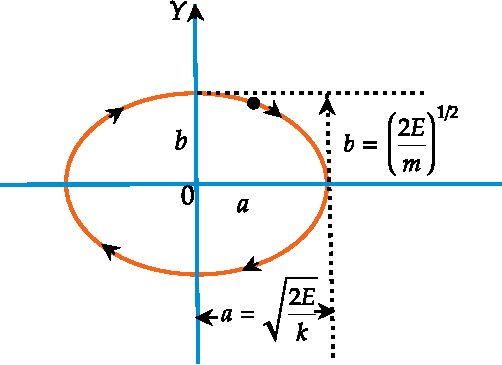
\includegraphics[height=5cm,width=8cm]{diagram-20220215-20220215103508-crop-crop}
	\caption{}
	\label{}
\end{figure}
This is well known equation of ellipse with center at the origin,semi-major axis $a=\sqrt{\frac{2E}{k}}$ and semi minor axis $b=\sqrt{\frac{2E}{m}}$\\
The phase trajectory of a differential equation is a definite ellipse for a given value of total energy E.Different ellipse in a phase plane corresponds to different vauesof total energy of the system.The equation $y=\dot{x}$ indicates that the representative point P(x,y) traverse the phase trajectory in clockwise sense.The centre of any ellipse x=0,y=0 is a singular point of the system.This singular point is enclosed by all trajectories.A singular of this type which is enclosed by all trajectories and approched by none is called a \textbf{vortex point}.The vortex point is position of stable equilibium of the system.\\
If $x=x_0,y=y_0$ at t=0 the time integral of the differential equation gives\\
$$x=\frac{y_0}{\omega}\sin \omega t+x_0\cos \omega t$$
$$y=y_0\cos \omega t-\omega x_0 \sin \omega t$$ 
With $ \omega=\sqrt{\frac{k}{m}}$.These are parametric equation of the ellipse.\\
The period of revolution of representative point \\
$$T=\frac{2 \pi }{\omega}=2\pi \sqrt{\frac{m}{k}}$$
\textbf{2-A Periodic Motion}\\
Consider a particle of mass $m$ being repulsed from the origin along $X$ axis by a force proportional to its distance from the origin.\\
$F \infty x$ or $F=k x$, where $k$ is a constant.\\
From Newton's second law $F=m \frac{d^{2} x}{d t^{2}}$, therefore equation of motlon becomes\\
$\therefore \qquad m \frac{d^{2} x}{d t^{2}}=k x $\\
\begin{equation}
\text { or }  \frac{d^{2} x}{d t^{2}}=\frac{k}{m} x \text { or } \frac{d^{2} x}{d t^{2}}=a^{2} x\label{psd01}
\end{equation}
where \qquad
$a^{2}=\frac{k}{m}$\\
Equation (\ref{psd01}) is equivalent to two differential equations of first order as
$$
y=\frac{d x}{d t}, \quad \frac{d y}{d t}=a^{2} x
$$
Dividing these equations the phase trajectories are given by the equations
$$
\begin{aligned}
\frac{d y}{d x} &=\frac{a^{2} x}{y} \\
\Rightarrow \quad y d y &-a^{2} x d x=0
\end{aligned}
$$
Integrating we get
\begin{equation}
$$
y^{2}-a^{2} x^{2}=C
$$
\end{equation}
\begin{figure}[H]
	\centering
	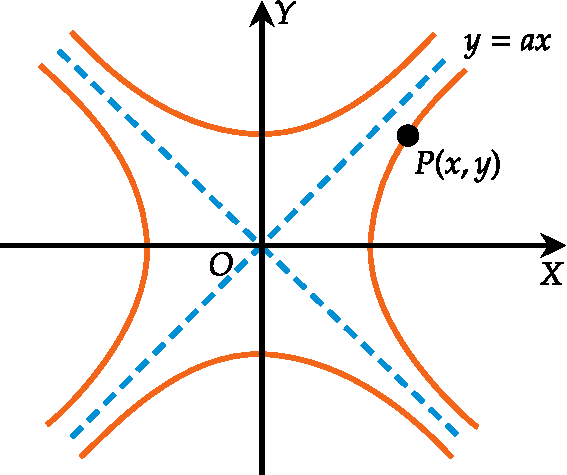
\includegraphics[height=4cm,width=5cm]{diagram-20220215-crop}
\end{figure}
where $C$ is a constant. This equation represents a hyperbola in the phase plane. Different values of $C$ correspond to different hyperbolas, whose two asymptotes are
$$
y=\pm a x .
$$
The origin $O$ is a singular point of a special type called the saddle point. In this case, there are two special trajectories that pass through the singular point (for which $C=0$ ). The motion of the representative point $P(x, y)$ along the trajectories that approach the saddle point is asymptotic with time $t$. The trajectories in the neighbourhood of a saddle point represent the possible motions that occur in the neighbourhood of a point of unstable equilibrium.\\
\textbf{3-Motion of a Damped Oscillator}\\
The differential equation of a damped harmonic oscillator with coefficient of damping ' $b$ ' is" given by
$$
\frac{m d^{2} x}{d t^{2}}=-b \frac{d x}{d t}-k x
$$
where $k$ is spring factor. This equation may be written as
$$
\begin{array}{l}
\frac{d^{2} x}{d t^{2}}+\frac{b}{m} \frac{d x}{d t}+\frac{k}{m} x=0 \\
\frac{d^{2} x}{d t^{2}}+2 r \frac{d x}{d t}+\omega_{0}^{2} x=0
\end{array}
$$
or\\
\begin{equation}
\text{where }\quad 2 r=\frac{b}{m}\text{ and }\omega_{0}^{2}=\frac{k}{m} \label{psd02}\\
\end{equation}
This equation is equivalent to two differential equations of first order given by
and
$$
\left.\begin{array}{l}
y=\frac{d x}{d t} \\
\frac{d y}{d t}=-\left(2 r y+\omega_{0}^{2} x\right)
\end{array}\right\}
$$
Dividing these equations, we get the equation of phase trajectory as
$$
\frac{d y}{d x}=-\frac{2 r y+\omega_{0}{ }^{2} x}{y}
$$
\textbf{Case (i) Underdamped case}\\
If $r^{2}<\omega_{0}{ }^{2}$, the motion of particle is damped oscillatory motion. Substituting $\omega=\sqrt{\omega_{0}{ }^{2}-r^{2}}$\\
The general solution of equation (\ref{psd02}) is 
$$x=A e^{-r t} \cos (\omega t+\phi)$$
$$y=\dot{x}=-A e^{-r t}[r \cos (\omega t+\phi)+\omega \sin (\omega t+\phi)\}$$where $A$ and $\phi$ are arbitrary constants.
\begin{figure}[H]
	\centering
	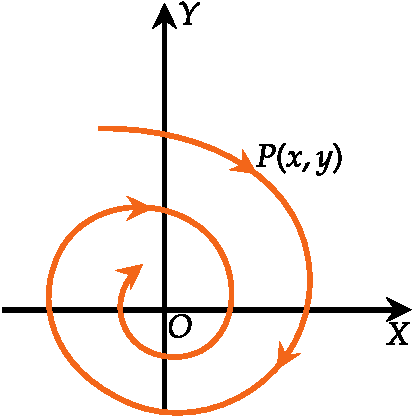
\includegraphics[height=4cm,width=4cm]{diagram-20220215(2)-crop}
	\caption{}
	\label{}
\end{figure}
These equations represent family of spirals; one spiral is shown in Figure . The origin $O$ is a singular point called the focal point. The representative point $P(x, y)$ spirals to approach the focal point at origin in an asymptotic manner. In this case the focal point at origin is a point of stable cquilibrium.\\
The representative point spirals to approach the focal point in an infinite number of times about it, so we may conclude that it does not approach $O$ with a definite direction.\\
\textbf{Case (ii) Overdamped Motion. }\\
If damping is large, then $r^{2}>\omega_{0}^{2}$ and motion is not oscillatory and is called overdamped motion.\\
Let
$$
\omega=\sqrt{r^{2}-\omega_{0}^{2}}
$$
In this case the general solution of equation $(\ref{psd02})$ is expressed as \\
\begin{equation}
\text{and}\qquad
\left.\begin{array}{l}
\quad x(t)=A e^{-\pi} \cosh (\omega t+\phi) \\
y(t)=\hat{x}(t)=A e^{-r t}[\omega \sinh (\omega t+\phi)-r \cosh (\omega t+\phi)]
\end{array}\right\}\label{psd03}
\end{equation}
\begin{figure}[H]
	\centering
	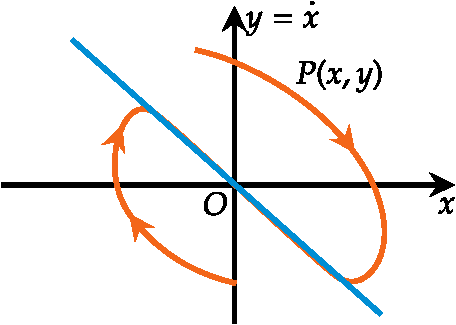
\includegraphics[height=3cm,width=5cm]{diagram-20220215(1)-crop}
	\caption{}
	\label{}
\end{figure}
where $A$ and $\phi$ are constants. Equations (\ref{psd03}) represents the phase trajectories of overdamped oscillator. A typical trajectory is shown in Figure  the origin $O$ is a singular point. The phase trajectories are such that the representative point $P(x, y)$ approaches towards the singular point with a definite direction; such a singular point is called a node or nodal point. The nodal point $O$ is the position of stable equilibrium. The four types of singular points are listed in the following table :\\\\
\begin{tabular}{|l|l|l|l|}
	\hline Name of singular point & \multicolumn{1}{|c|}{ Type of motion } & \multicolumn{1}{|c|}{ Type of equilibrium } & Approach \\
	\hline 1. Vortex point & Oscillatory & Stable & none \\
	\hline 2. Saddle point & Aperiodic & Unstable & only along asymptotes \\
	\hline 3. Focal point & Damped oscillatory & Stable & with no definite direction \\
	\hline 4. Nodal point & Aperiodic & Stable & with a definite direction \\
	\hline
\end{tabular}
\begin{example}\textbf{Falling body in a gravitational field}\\
Let $x$ denote the height at some time $t$. The force equation may be written as two first order equations:
$$
\begin{gathered}
\frac{d x}{d t}=v_{x}(x, y)=y \\
\frac{d y}{d t}=v_{y}(x, y)=-g
\end{gathered}
$$
where $g$ is the acceleration due to gravity. Thus the velocity field is given by,
$$
\vec{v}=(y,-g)
$$
Since $g$ is never zero there are no fixed points in this system. The equation of the phase curve and its solution is	\\
$$
\frac{d y}{d x}=-\frac{g}{y} \Rightarrow x=x_{0}-y^{2} / 2 g
$$
where $x_{0}$ is the height at $t=0$. The phase curves are therefore parabolas as shown in the figure below.\\
\begin{figure}[H]
	\centering
	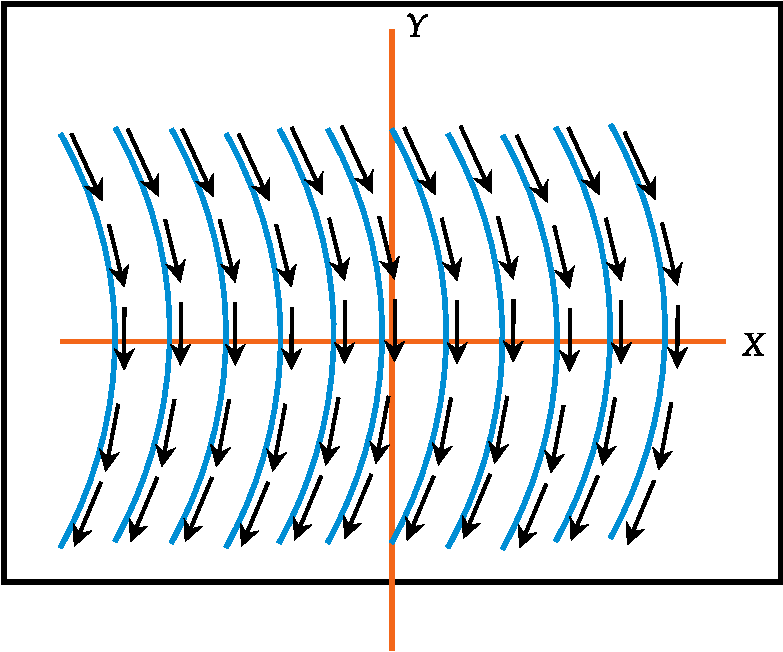
\includegraphics[height=4cm,width=5cm]{diagram-20220215(6)-crop}
	\caption{}
	\label{}
\end{figure}
Different phase curves correspond to different initial conditions. The phase flows are characterised by the arrows of length and orientation given by
$$
|\vec{v}|=\sqrt{y^{2}+g^{2}}, \quad \tan (\theta)=-g / y
$$
\end{example}


\section{Linear stability analysis}
We shall confine our analysis to 2 nd order autonomous systems, for example, motion of a particle in one dimension or systems with one degree of freedom (dof). The motivation, as we shall see below, for a general stability analysis is to derive the local and where possible global properties of a dynamical system qualitatively, that is, without actually solving the evolution equations.
For an autonomous system of order 2 we have\\
$$\begin{aligned}
	&\frac{d x}{d t}=v_{x}(x, y) \\
	&\frac{d y}{d t}=v_{y}(x, y)
\end{aligned}$$
where $(x, y)$ define the state of the system in the phase space. We shall assume that $\vec{v}$ is some function of $x, y$ which may be non-linear and therefore have many roots. The fixed point is defined through
$$
v_{x}\left(x_{k}, y_{k}\right)=0=v_{y}\left(x_{k}, y_{k}\right)
$$
and there may be many solutions. The nature of fixed points and the phase flows in the neighbourhood will be determined by the derivatives evaluated at the fixed point.
Consider one such fixed point $\left(x_{0}, y_{0}\right)$. The stability around this fixed point may be obtained by giving a small displacement around the fixed point:
$$
\begin{aligned}
&x(t)=x_{0}+\delta x(t) \\
&y(t)=y_{0}+\delta y(t)
\end{aligned}
$$
Now Taylor expand the velocity function $\vec{v}$ around the fixed point.
$$
\begin{aligned}
&v_{x}(x, y)=v_{x}\left(x_{0}, y_{0}\right)+\left.\frac{\partial v_{x}}{\partial x}\right|_{x_{0}, y_{0}} \delta x+\left.\frac{\partial v_{x}}{\partial y}\right|_{x_{0}, y_{0}} \delta y+\ldots \\
&v_{y}(x, y)=v_{y}\left(x_{0}, y_{0}\right)+\left.\frac{\partial v_{y}}{\partial x}\right|_{x_{0}, y_{0}} \delta x+\left.\frac{\partial v_{y}}{\partial y}\right|_{x_{0}, y_{0}} \delta y+\ldots
\end{aligned}
$$
By definition the first term is zero since $\left(x_{0}, y_{0}\right)$ is a fixed point. For an infinitesimal variation in $(\delta x, \delta y)$ we may linearise the equations of motion-
$$
\left(\begin{array}{c}
d x / d t \\
d y / d t
\end{array}\right)=\left(\begin{array}{c}
d \delta x / d t \\
d \delta y / d t
\end{array}\right)=\left(\begin{array}{ll}
V_{x x} & V_{x y} \\
V_{y x} & V_{y y}
\end{array}\right)\left(\begin{array}{l}
\delta x \\
\delta y
\end{array}\right)
$$
or in a short form, and shifting the origin to $\left(x_{0}, y_{0}\right)$,
$$
\frac{d \delta \vec{r}}{d t}=A \delta \vec{r}
$$
where $A$ is a $2 \times 2$ matrix given by,
$$
A=\left(\begin{array}{ll}
\frac{\partial v_{x}}{\partial x} & \frac{\partial v_{x}}{\partial y} \\
\frac{\partial v_{y}}{\partial x} & \frac{\partial v_{y}}{\partial y}
\end{array}\right)_{x_{0}, y_{0}}
$$
The local stability analysis is best done in the eigenbasis or in some other convenient basis which we shall call the Standard Basis.

If the system is already linear the above analysis is globally, not just locally, valid since
$$
\begin{aligned}
&\frac{d x}{d t}=v_{x}(x, y)=a x+b y \\
&\frac{d y}{d t}=v_{y}(x, y)=c x+d y
\end{aligned}
$$
and the matrix $A$ is given by,
$$
A=\left(\begin{array}{ll}
a & b \\
c & d
\end{array}\right)
$$
However, we need not restrict the analysis only to linear systems. Consider the change of basis
$$
M\left(\begin{array}{l}
\delta x \\
\delta y
\end{array}\right)=\left(\begin{array}{l}
\delta X \\
\delta Y
\end{array}\right)
$$
such that
$$
B=M A M^{-1}=\left(\begin{array}{cc}
\lambda_{1} & 0 \\
0 & \lambda_{2}
\end{array}\right)
$$
where $\lambda_{i}$ are the eigenvalues of the stability matrix given by
$$
\begin{aligned}
&\lambda_{1}=\frac{1}{2}\left(\tau-\sqrt{\tau^{2}-4 \delta}\right) \\
&\lambda_{2}=\frac{1}{2}\left(\tau+\sqrt{\tau^{2}-4 \delta}\right)
\end{aligned}
$$
where
$$
\begin{gathered}
\tau=V_{x x}+V_{y y} \\
\delta=V_{x x} V_{y y}-V_{x y} V_{y x}
\end{gathered}
$$
are respectively the trace and the determinant of the stability matrix. The eigenvalues are real or complex depending on whether $\tau^{2} \geq 4 \delta$ or $\tau^{2}<4 \delta .$ We shall consider these cases separately.

In the transformed coordinates the linearised equations of motion and their solutions in the neighbourhood of the fixed point are given by
$$
\begin{aligned}
\delta \dot{X} &=\lambda_{1} \delta X \Rightarrow \delta X(t)=C_{1} \exp \left(\lambda_{1} t\right) \\
\delta \dot{Y} &=\lambda_{2} \delta Y \Rightarrow \delta Y(t)=C_{2} \exp \left(\lambda_{2} t\right)
\end{aligned}
$$
The equation for the phase curve is
$$
\left(\delta X / C_{1}\right)^{\lambda_{2}}=\left(\delta Y / C_{2}\right)^{\lambda_{1}}
$$
\subsection{ Classification of the fixed points}
We use the properties of the eigenvalues to classify the fixed points. While in the first order systems motion either moves towards or away from the fixed point, the second order systems are richer in the sense there is much more variety in the nature of fixed points.\\
\begin{enumerate}
	\item \textbf{$\text { Stable Node, } \lambda_{1}, \lambda_{2}<0$}
	$$
	\delta X, \delta Y \rightarrow 0
	$$
	as $t \rightarrow \infty$\\
	If in particular $\lambda_{1}=\lambda_{2}<0$ and the equation is separable, $A=\lambda I$, it is called a stable star. (See Figure). If not a change of basis may be induced such that the matrix
	$$
	B=\left(\begin{array}{ll}
	\lambda & 0 \\
	c & \lambda
	\end{array}\right)
	$$
	or equivalently $c=0$ and $b \neq 0$. In this case
	$$
	\begin{gathered}
	\delta \dot{X}=\lambda \delta X \Rightarrow \delta X(t)=C_{1} \exp (\lambda t) \\
	\delta \dot{Y}=c \delta X+\lambda \delta Y \Rightarrow \delta Y(t)=\left(C_{2}+C_{1} c t\right) \exp (\lambda t)
	\end{gathered}
	$$
	For $\lambda<0$ this is called an improper node.
	\item \textbf{$\text { Unstable Node, } \lambda_{1}, \lambda_{2}>0 \text {. }$}
	$$\delta X, \delta Y \rightarrow \infty$$
	as $t \rightarrow \infty .$ If in particular $\lambda_{1}=\lambda_{2}>0$ and $A=\lambda I$ it is called a unstable star.
	(See Figure).\\
	\begin{figure}[H]
		\centering
		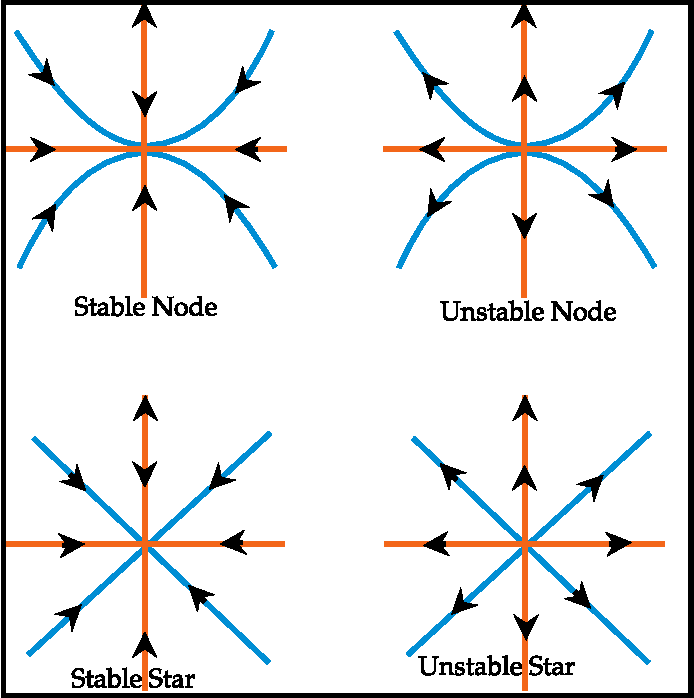
\includegraphics[height=7cm,width=8cm]{diagram-20220215(3)-crop}
		\caption{}
		\label{}
	\end{figure}
	\item \textbf{$\text { Hyperbolic fixed point, } \lambda_{1}>0, \lambda_{2}<0 $}
	$$|\delta X| \rightarrow \infty,|\delta Y| \rightarrow 0$$
	as $t \rightarrow \infty$. This fixed point is also called a saddle point. These are rather special. If in particular the system has only one fixed point then the saddle point divides the phase space into four quadrants, each of which is an invariant subspace. That is a trajectory starting in one of the quadrants remains confined to the same quadrant for all times. These regions are separated by trajectories heading towards or away from the fixed point. The set of points along these trajectories are called invariant manifolds.\\\\
	Next consider the case when the eigenvalues are complex.
	\item \textbf{$\text { Stable spiral fixed point, } \lambda_{1}=-\alpha+i \beta, \lambda_{2}=-\alpha-i \beta \text { where } \alpha, \beta>0$}
	Correspondingly we have,
	$$
	\delta X=C_{1} e^{-\alpha t+i \beta t}, \quad \delta Y=C_{2} e^{-\alpha t-i \beta t}
	$$
	By a change of basis the solutions may be written as
	$$
	\begin{gathered}
	\delta X^{\prime}=e^{-\alpha t}\left(C_{1} \cos \theta t+C_{2} \sin \theta t\right) \\
	\delta Y^{\prime}=e^{-\alpha t}\left(-C_{1} \sin \theta t+C_{2} \cos \theta t\right)
	\end{gathered}
	$$
	The fixed point is called the spiral fixed point by looking at the behaviour of the real and imaginary parts as shown in the figure or the solutions given above explicitly in terms of the rotation angle $\theta$. It is stable since for large times the system tends towards the fixed point.
	\item \textbf{$\text { Unstable spiral fixed point, } \lambda_{1}=\alpha+i \beta, \lambda_{2}=\alpha-i \beta \text { where } \alpha, \beta>0 $}
	Correspondingly we have,
	$$
	\delta X=C_{1} e^{\alpha t+i \beta t}, \quad \delta Y=C_{2} e^{\alpha t-i \beta t}
	$$
	The fixed point is unstable since for large times the system moves away from the fixed point.
	\item \textbf{$\text { Elliptic fixed point, } \lambda_{1}=i \omega=-\lambda_{2}$}
 Correspondingly we have,\\
 $$\delta X=C_{1} e^{i \omega t}, \quad \delta Y=C_{2} e^{-i \omega t}$$
 The system is confined to ellipses around the fixed point- each ellipse corresponds to a given initial condition.\\
 \begin{figure}[H]
 	\centering
 	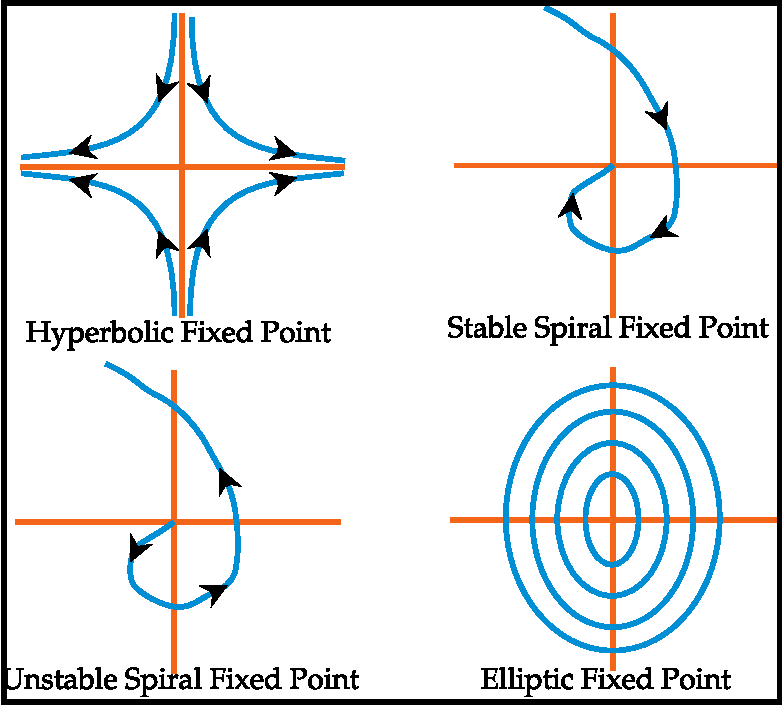
\includegraphics[height=7cm,width=8cm]{diagram-20220215(4)-crop}
 	\caption{}
 	\label{}
 \end{figure}
\end{enumerate}
\subsection{Limit cycle}
In first-order systems all motions tend to fixed points or to infinity. In second order systems, in addition to fixed points, the system may also exhibit \textbf{a limit cycle} which is a closed trajectory encircling the fixed point. The trajectories within and outside tend towards the limiting trajectory as time $t \rightarrow \infty .$ Such a behaviour occurs typically in systems that are oscillatory. A rigorous analysis of limit cycles, their occurrence and stability is beyond the scope of these lectures.\\
\begin{figure}[H]
	\centering
	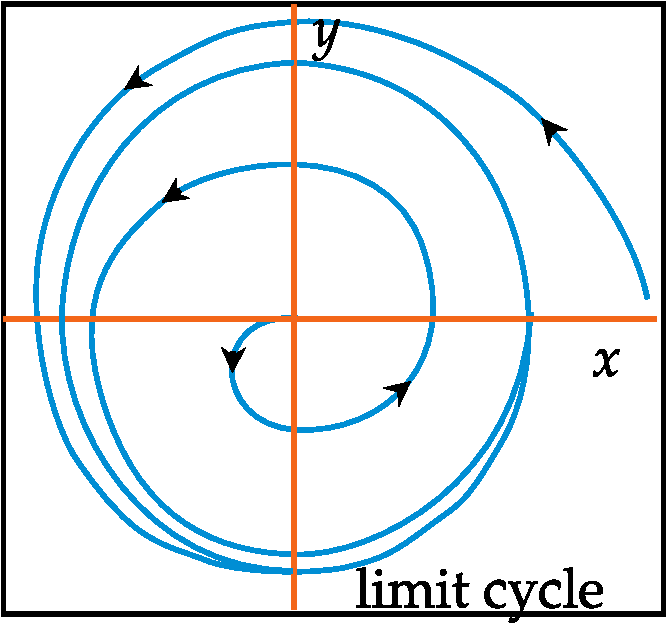
\includegraphics[height=4cm,width=5cm]{diagram-20220215(5)-crop}
	\caption{}
	\label{}
\end{figure}
 However, it may be noted that they occur in systems where the long-term motion of the system is limited to some finite region in the state space. Because of the no intersection theorem, it is entirely reasonable to assume that in this bounded region the trajectory either approaches a fixed point or a closed trajectory (cycle) as $t \rightarrow \infty$. Indeed this is the content of the famous \textbf{Poincare-Bendixson Theorem.}
\section{Application to Commonly-Encountered Systems}
\subsection{ Simple Pendulum}
In this example, because the Hamiltonian is constant and equal to the energy of the system, the easiest way to generate a phase plot is to derive the Hamiltonian in terms of $\boldsymbol{p}$ and $\boldsymbol{q}$. The Hamiltonian of the simple pendulum illustrated in Figure 1, consisting of a mass $m$ suspended by a massless string of length $l$ is given by:
$$
H(\theta, p)=T+V=\frac{p^{2}}{2 m l^{2}}-m g l \cos \theta
$$
In this particular case, it's obvious that $\theta=q$, the generalized coordinate and the Hamiltonian is timeindependent and is equal to the total energy of the pendulum system.\\
Figure 2 is the phase-space representation of the motion of the pendulum for four different values of the Hamiltonian or energy of the system.\\
 \par The innermost (green) curve or trajectory represents the motion of the pendulum for the lowest of the four energy levels. The pendulum has sufficient energy to swing through an angle of approximately $\pm \frac{\pi}{2}$ and obviously has the lowest maximum value of momentum. As time advances, the phase point representing the instantaneous state of the pendulum system repeatedly traces out the green trajectory, one period represented by a single orbit.
The blue trajectory represents the motion of the pendulum with slightly higher energy than the green trajectory as demonstrated by the higher maximum value for the momentum and $\theta$.
The purple trajectory represents a higher energy than the blue or green and shows the swing angle $\theta$ approaching $\pm \pi$, the maximum swing angle while still retaining 'back and forth' motion.
The orange, outermost trajectory represents the highest of the four energy levels and clearly demonstrates that the pendulum is now rotating continuously in one direction (no longer exhibiting 'back and forth' motion) by virtue of the open trajectory. An obvious implication of the open trajectory is that the system's momentum never falls to zero and continues in the same direction without limit.\\
\begin{figure}[H]
	\centering
	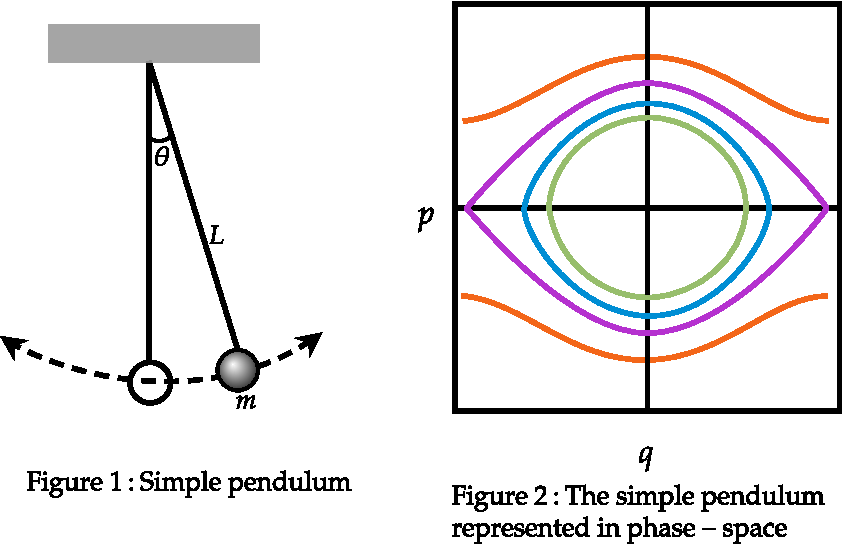
\includegraphics[height=6cm,width=10cm]{diagram-20220215(7)-crop}
	\caption{}
	\label{}
\end{figure}
The phase-space trajectory that represents the motion of the pendulum at the limit where the motion changes from 'back and forth' to continuous rotation is called the separatrix. The purple trajectory in figure 2 is very close in energy to the separatrix and is extremely close to it in shape.\\
\begin{note}
	$\text { Driven, damped SHO at resonance. }$\\
	\begin{figure}[H]
		\centering
		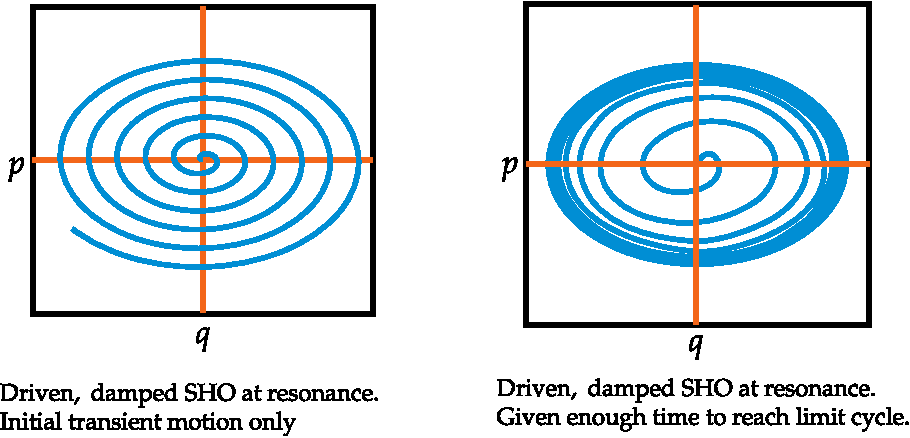
\includegraphics[height=6cm,width=10cm]{diagram-20220215(11)-crop}
		\caption{}
		\label{}
	\end{figure}
\end{note}
\subsection{Damped Mass on a Spring}
In this example, a mass $m$ attached to the free end of a spring with spring constant $k$ is subject to a damping force $\gamma$ as shown in figure 4 . A mass on an ideal spring exhibits simple harmonic oscillations and is described by the following differential equation:
$$
m \frac{d^{2} \boldsymbol{x}}{d t^{2}}+k \boldsymbol{x}=0
$$
When the oscillations are subject to a damping force, the motion is described by:
$$
m \frac{d^{2} \boldsymbol{x}}{d t^{2}}+\gamma \frac{d \boldsymbol{x}}{d t}+k \boldsymbol{x}=0
$$
Solving this differential equation provides us with the generalized coordinate $\boldsymbol{x}(t)=\boldsymbol{q}$. The generalized momentum can then be determined from the derivative of $\boldsymbol{x}(t)$.\\
$$
\boldsymbol{p}=m \dot{\boldsymbol{x}}(t)
$$
The obvious difference between this example and the simple pendulum is that $\boldsymbol{p}$ and $\boldsymbol{q}$ are both timedependent.
Solving the differential equation for the damped motion to find $\boldsymbol{q}$ and then differentiating to obtain $\boldsymbol{p}$, the phase-plot shown in figure 5 can be generated.\\
\begin{figure}[H]
	\centering
	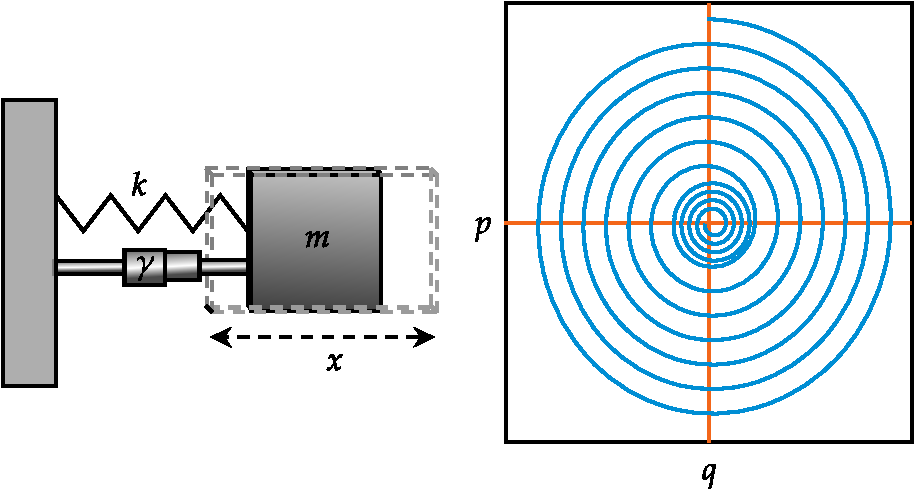
\includegraphics[height=6cm,width=10cm]{diagram-20220215(8)-crop}
	\caption{figure 4 and 5}
	\label{}
\end{figure}
The phase plot clearly shows how the momentum and displacement diminish with time resulting in a dramatic spiral trajectory. Without the damping force, the trajectory would be a closed ovoid similar to that for the simple pendulum with small oscillations. Figure 5 also shows how the damping force is reduced with diminishing momentum, a fact that is easily implied from the velocity term of the differential equation $\gamma \frac{d x}{d t}$.
\newpage
\begin{abox}
	Practice set 1 
	\end{abox}
\begin{enumerate}
\begin{minipage}{\textwidth}
	\item The trajectory on the $z p_{z}$ - plane (phase-space trajectory) of a ball bouncing perfectly elastically off a hard surface at $z=0$ is given by approximately by (neglect friction):
	\exyear{NET JUNE 2011}
\end{minipage}
\begin{tasks}(2)
	\task[\textbf{A.}]\begin{figure}[H]
		\centering
		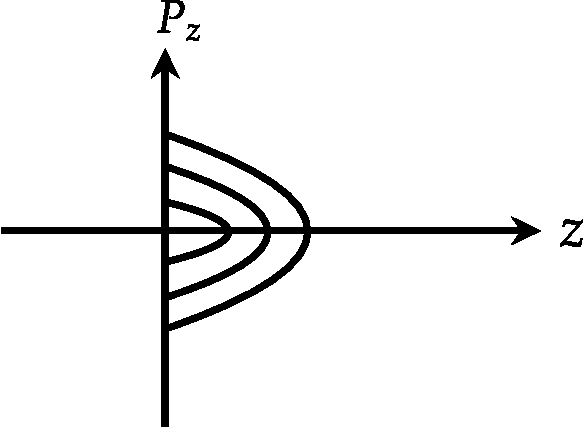
\includegraphics[height=3cm,width=5cm]{diagram-20210926(3)-crop}
	\end{figure}
	\task[\textbf{B.}]\begin{figure}[H]
		\centering
		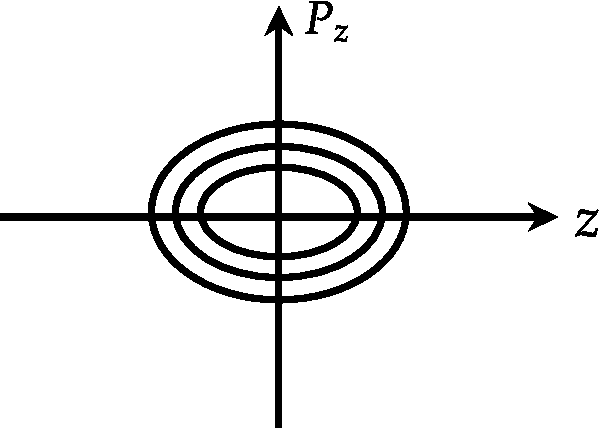
\includegraphics[height=3cm,width=5cm]{diagram-20210926(4)-crop}
	\end{figure}
	\task[\textbf{C.}]\begin{figure}[H]
		\centering
		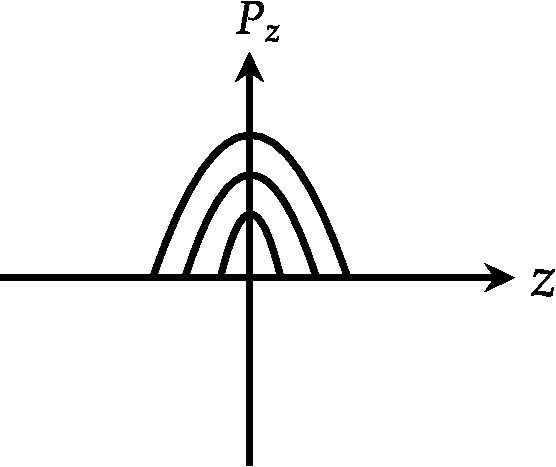
\includegraphics[height=3cm,width=5cm]{diagram-20210926(5)-crop}
	\end{figure}
	\task[\textbf{D.}]\begin{figure}[H]
		\centering
		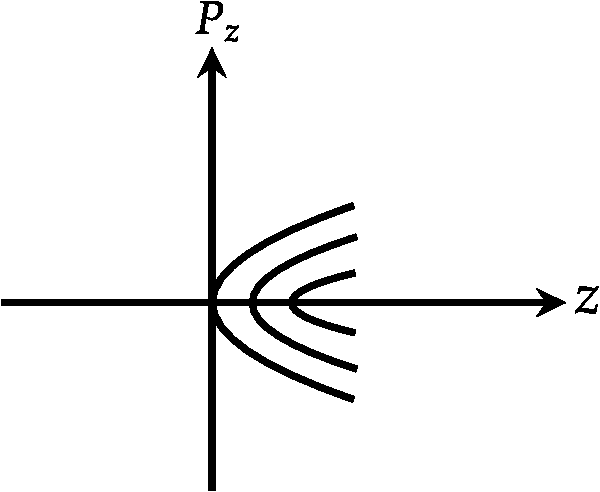
\includegraphics[height=3cm,width=5cm]{diagram-20210926(6)-crop}
	\end{figure}
\end{tasks}
\begin{minipage}{\textwidth}
	\item The bob of a simple pendulum, which undergoes small oscillations, is immersed in water. Which of the following figures best represents the phase space diagram for the pendulum?
	\exyear{NET JUNE 2012}
\end{minipage}
\begin{tasks}(2)
	\task[\textbf{A.}]\begin{figure}[H]
		\centering
		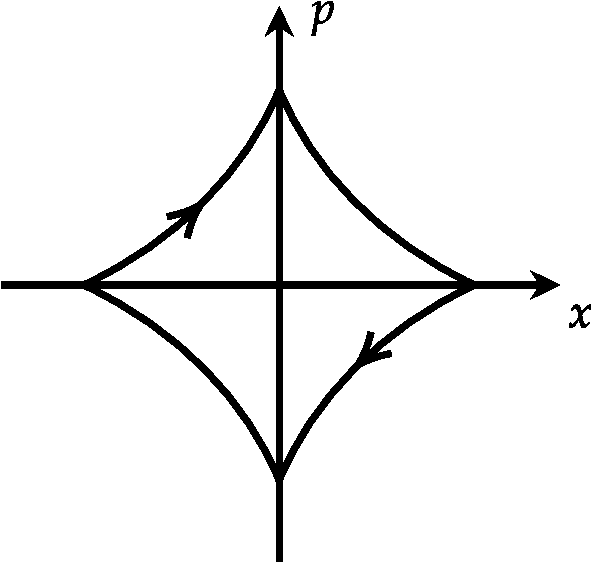
\includegraphics[height=3cm,width=5cm]{diagram-20210926(7)-crop}
	\end{figure}
	\task[\textbf{B.}]\begin{figure}[H]
		\centering
		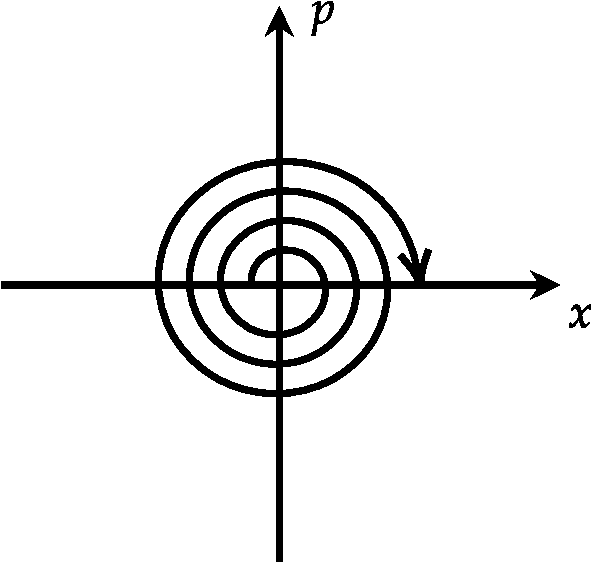
\includegraphics[height=3cm,width=5cm]{diagram-20210926(8)-crop}
	\end{figure}
	\task[\textbf{C.}]\begin{figure}[H]
		\centering
		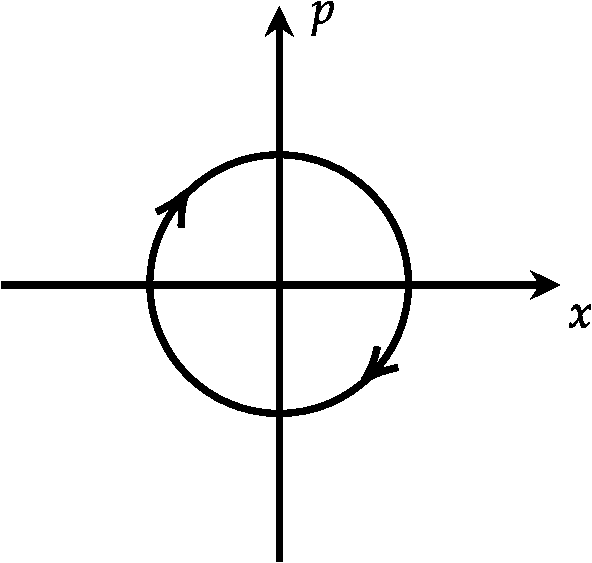
\includegraphics[height=3cm,width=5cm]{diagram-20210926(9)-crop}
	\end{figure}
	\task[\textbf{D.}]\begin{figure}[H]
		\centering
		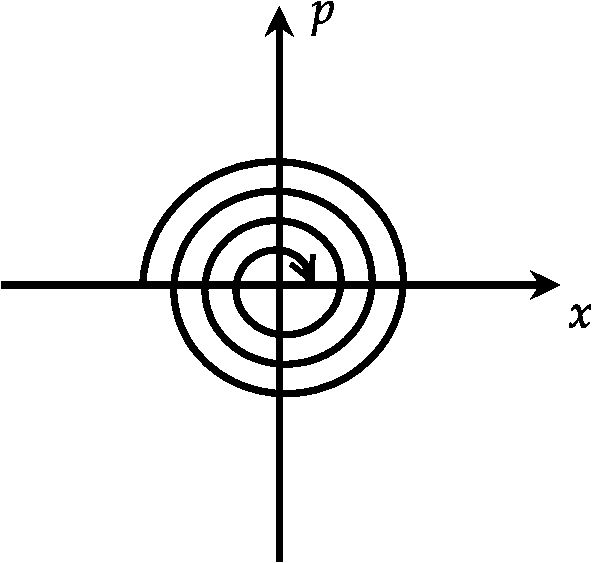
\includegraphics[height=3cm,width=5cm]{diagram-20210926(10)-crop}
	\end{figure}
\end{tasks}
\begin{minipage}{\textwidth}
	\item Which of the following set of phase-space trajectories is not possible for a particle obeying Hamilton's equations of motion?
	\exyear{NET DEC 2012}
\end{minipage}
\begin{tasks}(2)
	\task[\textbf{A.}]\begin{figure}[H]
		\centering
		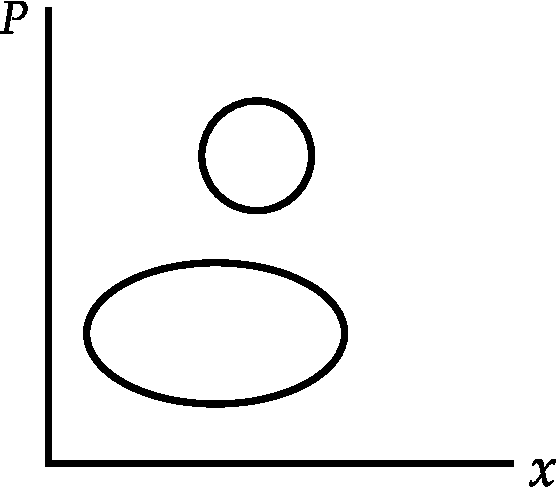
\includegraphics[height=3cm,width=5cm]{diagram-20210926(13)-crop}
	\end{figure}
	\task[\textbf{B.}]\begin{figure}[H]
		\centering
		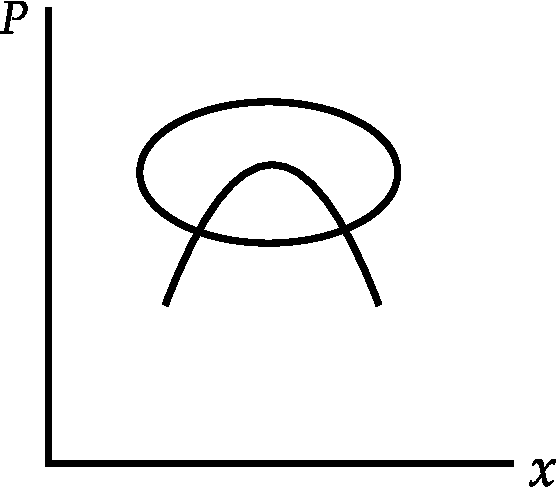
\includegraphics[height=3cm,width=5cm]{diagram-20210926(14)-crop}
	\end{figure}
	\task[\textbf{C.}]\begin{figure}[H]
		\centering
		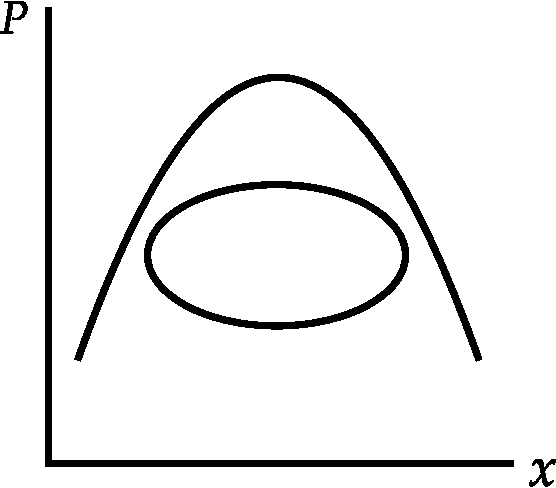
\includegraphics[height=3cm,width=5cm]{diagram-20210926(15)-crop}
	\end{figure}
	\task[\textbf{D.}]\begin{figure}[H]
		\centering
		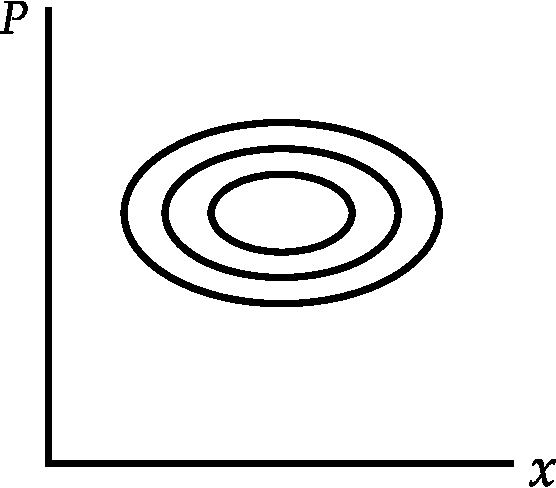
\includegraphics[height=3cm,width=5cm]{diagram-20210926(16)-crop}
	\end{figure}
\end{tasks}
\begin{minipage}{\textwidth}
	\item The Hamiltonian of a classical particle moving in one dimension is $H=\frac{p^{2}}{2 m}+\alpha q^{4}$ where $\alpha$ is a positive constant and $p$ and $q$ are its momentum and position respectively. Given that its total energy $E \leq E_{0}$ the available volume of phase space depends on $E_{0}$ as
	\exyear{NET DEC 2014}
\end{minipage}
\begin{tasks}(2)
	\task[\textbf{A.}] $E_{0}^{3 / 4}$
	\task[\textbf{B.}]$E_{0}$
	\task[\textbf{C.}]$\sqrt{E_{0}}$
	\task[\textbf{D.}]is independent of $E_{0}$
\end{tasks}
\begin{minipage}{\textwidth}
	\item Which of the following figures is a schematic representation of the phase space trajectories (i.e., contours of constant energy) of a particle moving in a one-dimensional potential $V(x)=\frac{-1}{2} x^{2}+\frac{1}{4} x^{4}$
	\exyear{NET JUNE 2015}
\end{minipage}
\begin{tasks}(2)
	\task[\textbf{A.}]\begin{figure}[H]
		\centering
		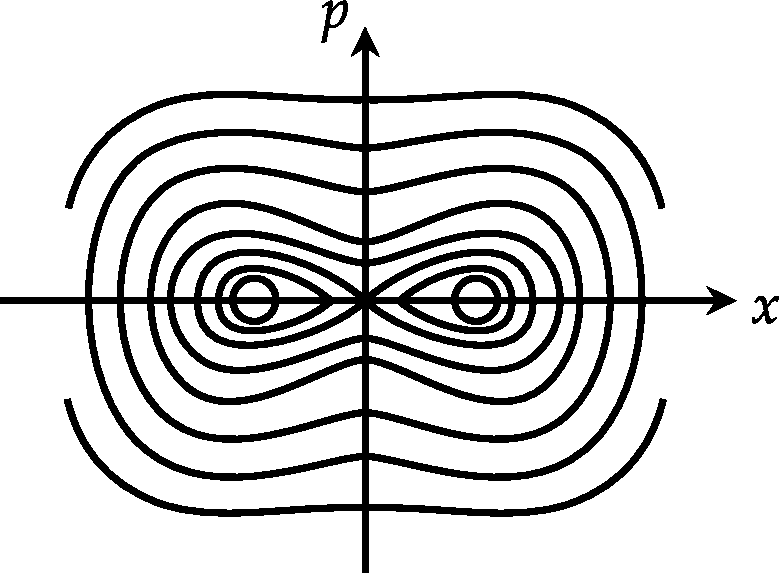
\includegraphics[height=3cm,width=5cm]{diagram-20210926(24)-crop}
	\end{figure}
	\task[\textbf{B.}]\begin{figure}[H]
		\centering
		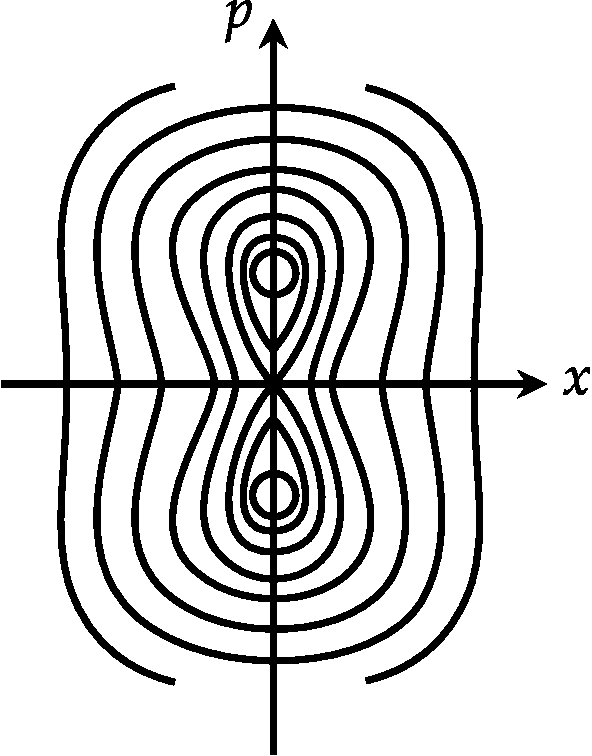
\includegraphics[height=3cm,width=5cm]{diagram-20210926(25)-crop}
	\end{figure}
	\task[\textbf{C.}]\begin{figure}[H]
		\centering
		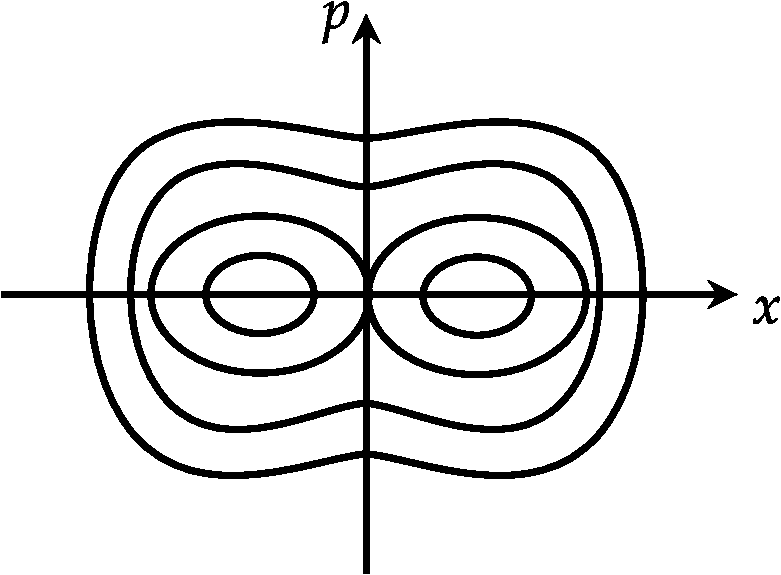
\includegraphics[height=3cm,width=5cm]{diagram-20210926(26)-crop}
	\end{figure}
	\task[\textbf{D.}]\begin{figure}[H]
		\centering
		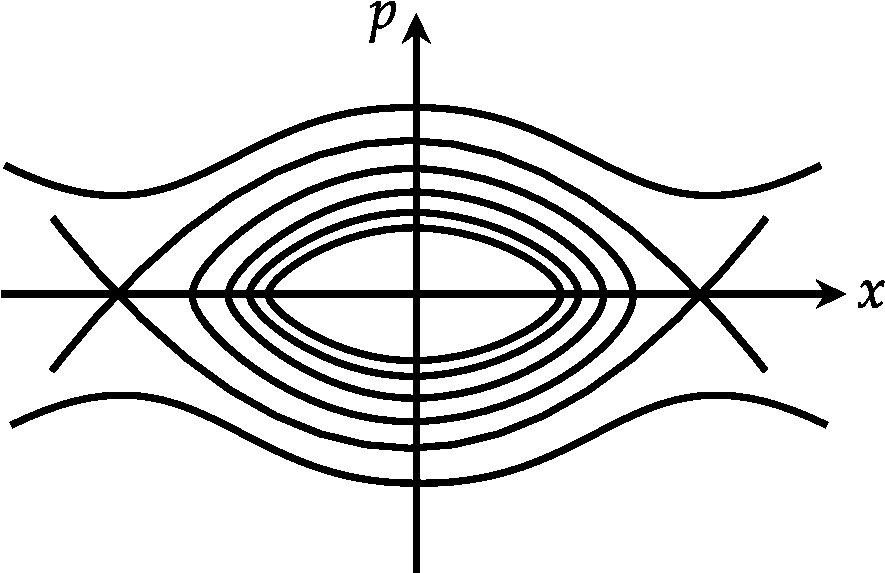
\includegraphics[height=3cm,width=5cm]{diagram-20210926(27)-crop}
	\end{figure}
\end{tasks}
\begin{minipage}{\textwidth}
	\item A particle moves in one dimension in a potential $V(x)=-k^{2} x^{4}+\omega^{2} x^{2}$ where $k$ and $\omega$ are constants. Which of the following curves best describes the trajectories of this system in phase space?
	\exyear{NET DEC 2017}
\end{minipage}
\begin{tasks}(2)
	\task[\textbf{A.}]\begin{figure}[H]
		\centering
		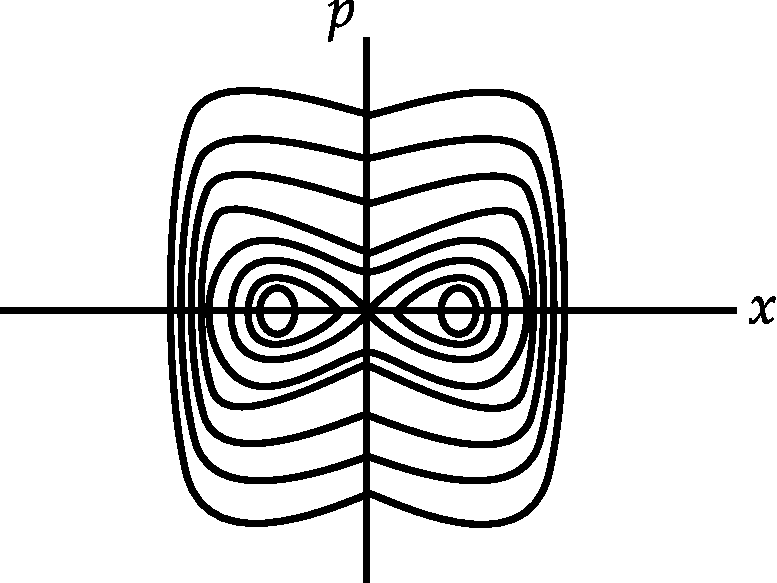
\includegraphics[height=3cm,width=5cm]{diagram-20210926(42)-crop}
	\end{figure}
	\task[\textbf{B.}]\begin{figure}[H]
		\centering
		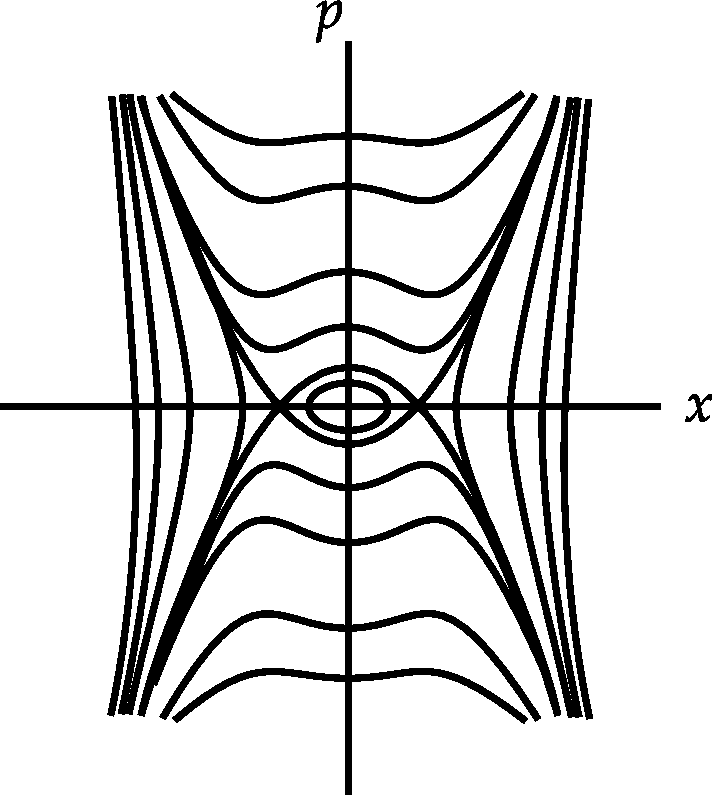
\includegraphics[height=3cm,width=5cm]{diagram-20210926(43)-crop}
	\end{figure}
	\task[\textbf{C.}]\begin{figure}[H]
		\centering
		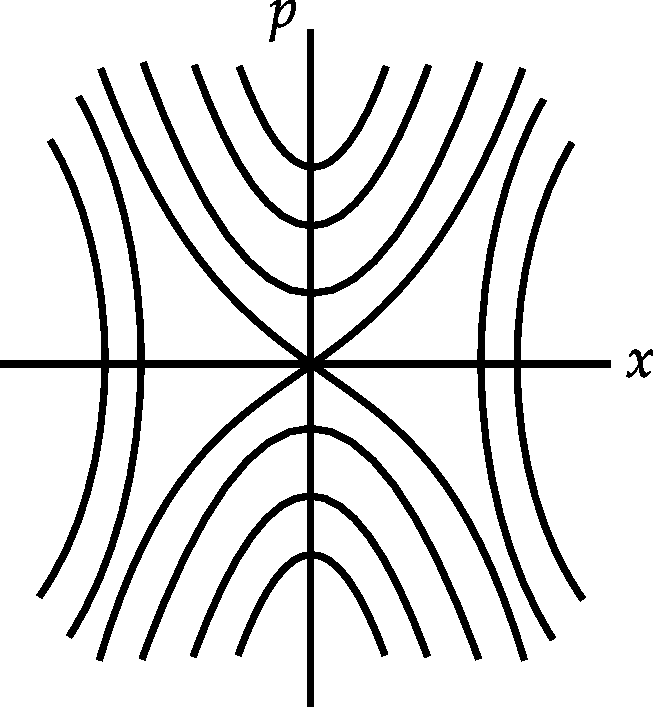
\includegraphics[height=3cm,width=5cm]{diagram-20210926(44)-crop}
	\end{figure}
	\task[\textbf{D.}]\begin{figure}[H]
		\centering
		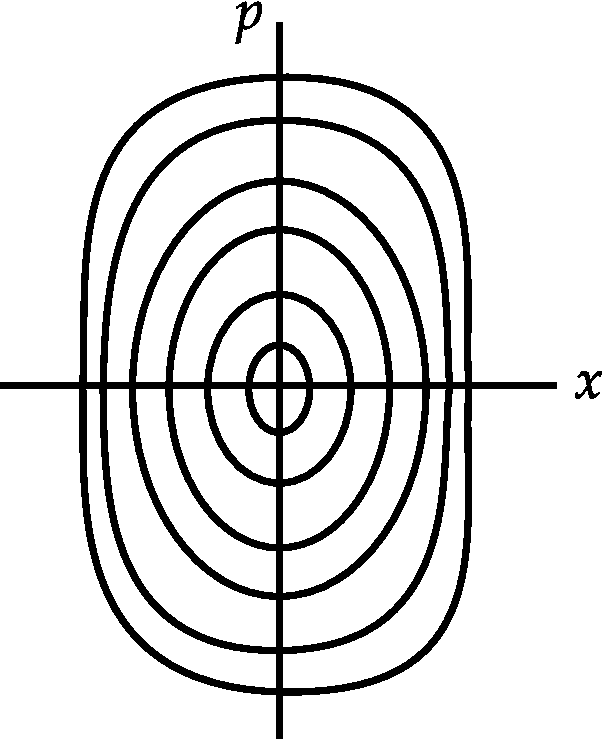
\includegraphics[height=3cm,width=5cm]{diagram-20210926(45)-crop}
	\end{figure}
\end{tasks}
\end{enumerate}
\colorlet{ocre1}{ocre!70!}
\colorlet{ocrel}{ocre!30!}
\setlength\arrayrulewidth{1pt}
\begin{table}[H]
	\centering
	\arrayrulecolor{ocre}
	
	\begin{tabular}{|p{1.5cm}|p{1.5cm}||p{1.5cm}|p{1.5cm}|}
		\hline
		\multicolumn{4}{|c|}{\textbf{Answer key}}\\\hline\hline
		\rowcolor{ocrel}Q.No.&Answer&Q.No.&Answer\\\hline
		1&\textbf{a}&2&\textbf{d}\\\hline
		3&\textbf{b}&4&\textbf{a}\\\hline
		5&\textbf{a}&6&\textbf{c}\\\hline
	\end{tabular}
\end{table}
